\chapter{Architektur und Technologien}
\label{ch:Architektur und Technologien}
Dieses Kapitel beschreibt die verwendeten Technologien und die Architektur der Testbench. Aufgabe ist es ein Kommandozeilen-basiertes Programm zu entwickeln, das basierend auf gegebenen Konfigurations-Dateien die Testbench startet und die Simulation durchführt. Die beobachteten Ergebnisse sollen anschließend wiederum in Dateien geschrieben werden



\section{Technologien}
\label{sec:Architektur und Technologien:Technologien}
Die vorgegebene, zu verwendende Programmiersprache ist Java. Weiterhin wird das Java-basierte Spring-Framework\footnote{https://spring.io/} verwendet, da es einige nützliche Features wie \textit{Dependency Injection} oder Event-basierte Kommunikation bietet. Als Applikationsserver wird durch Spring implizit eine leichtgewichtige Variante von Tomcat benutzt. Für den Augenblick besitzt der Auto-Skalierer keine Benutzeroberfläche und läuft auf einem lokalen Rechner. Mit Hinblick auf die Zukunft, könnte die Testbench entweder als Web-Applikation gestaltet werden, oder aber eine Benutzeroberfläche erhalten und als Desktop-Anwendung laufen. In beiden Fällen unterstützt das Spring-Framework diesen Evolutionsschritt enorm, sodass beide Varianten mit geringem Aufwand umgesetzt werden können. \\
Die Konfigurationen für die Testbench liegen im neutralen JSON-Format\footnote{https://www.json.org/} vor, da dieses sehr einfach eingelesen werden kann. Die Eingabe der Workload erfolgt ebenfalls im JSON-Format. \\
Die Ausgabe-Informationen sind zeit-diskrete, strukturierte Werte weshalb das Tabellen-Format \textit{CSV} zur Speicherung verwendet wird.


\section{Architektur}
\label{sec:Architektur und Technologien:Architektur}
Wie in Sektion \ref{fig:BasicIdea} beschrieben besteht die Testbench aus verschiedenen Modulen, die miteinander kommunizieren müssen. Gleichzeitig ist es wünschenswert, die Module lose zu koppeln und austauschbar zu gestalten. Auch kann eine Informationsquelle bei der Testbench mehrere Informationssenken haben: Der Zustand der Infrastruktur muss periodisch an verschiedenste Komponenten gesendet werden wie zum Beispiel an die Module zur Aufzeichnung der diversen Metriken oder an den Auto-Skalierer. Weitere Informationssenken, die diese Information verarbeiten wollen, sollten dabei ohne größere Veränderung hinzugefügt werden können. Außerdem erzwingt die zeit-diskrete Simulation einen Taktgeber, der periodisch alle Komponenten über den nächsten Taktzyklus informiert. Direkte Kommunikation zwischen den jeweiligen Komponenten hätte dadurch einen nennenswerten Nachteil: Jede Komponente muss alle Komponenten kennen, mit denen sie kommunizieren muss. Im Falle des Taktgebers wären das sogar alle. \\
Event-basierte Architektur bietet einen Mechanismus, der das Versenden und Empfangen von Nachrichten entkoppelt. Damit ist es möglich die Module selbst zu entkoppeln und Nachrichtenaustausch über einen Event-Bus zu realisieren. Abbildung \ref{fig:EventBus} skizziert einen solchen Event Bus. Jede Komponente die eine Nachricht an andere Komponenten versenden möchte benötigt einen \textit{Event Publisher}, der eine (oder mehrere) Nachrichten versendet. Eine Nachricht hat dabei immer einen vordefinierten Typ. Jede Komponente die an dieser Nachricht interessiert ist, muss lediglich einen \textit{Event Listener} implementieren, der auf Nachrichten dieses Event-Typs hört. Falls eine weiteres Modul entwickelt wird, dass an bereits vorhandenen Nachrichtentypen interessiert ist (wie im Schaubild \textit{Event Listener 3}), so muss lediglich ein geeigneter Listener implementiert werden. Die anderen Module, vor allem die bereits implementierte Informationsquelle, muss dabei nicht verändert werden.  


%"l, b, r, t"
\begin{figure}[t]
	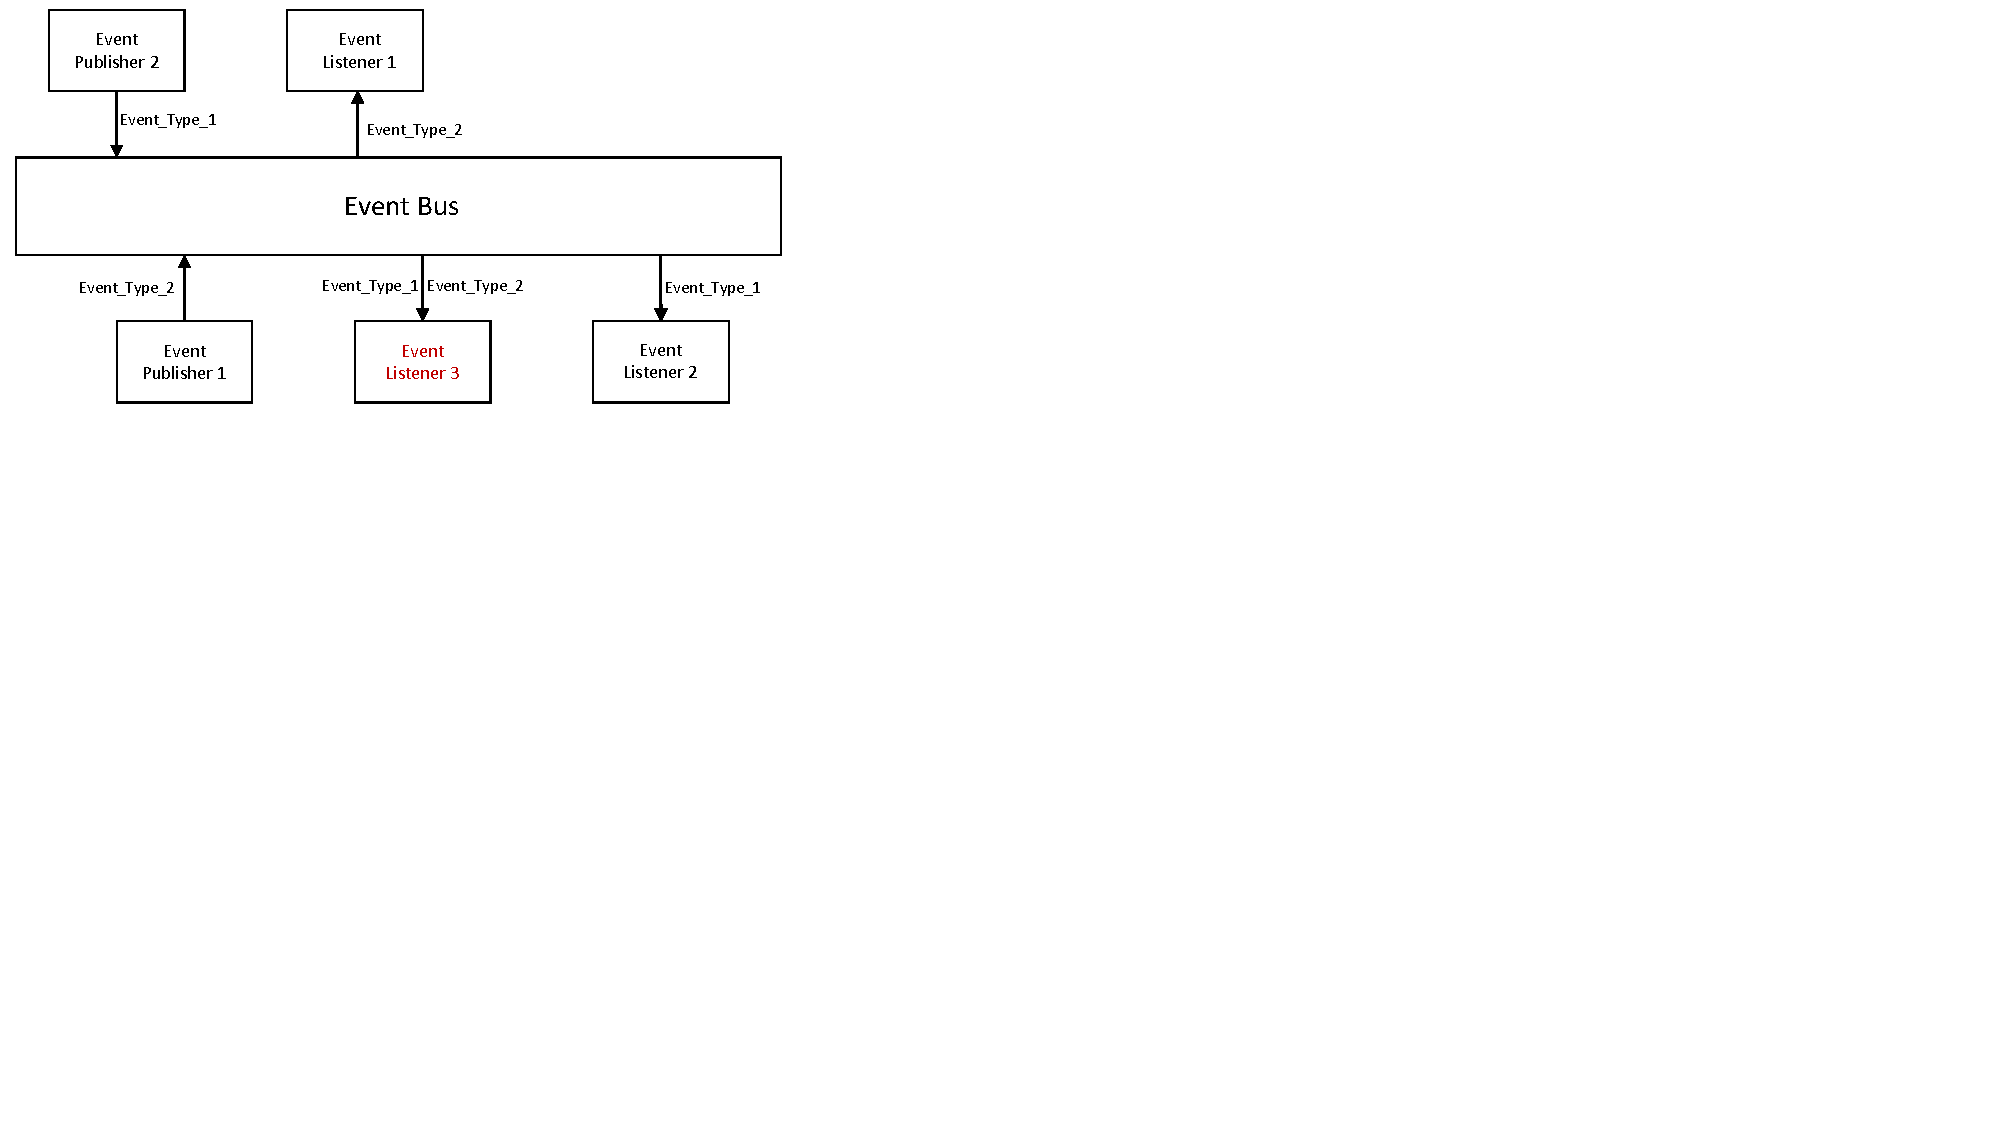
\includegraphics[width=\textwidth, trim={0cm 11.5cm 19cm 0cm}]{img/EventBus.pdf}
	\caption{Der Event-Bus}
	\label{fig:EventBus}
\end{figure}
